\section*{Exercice 152 -- Modélisation géométrique}
\setcounter{exo}{0}
%Ecole de l'air PSI 2002

On considère le système suivant. 
\begin{center}
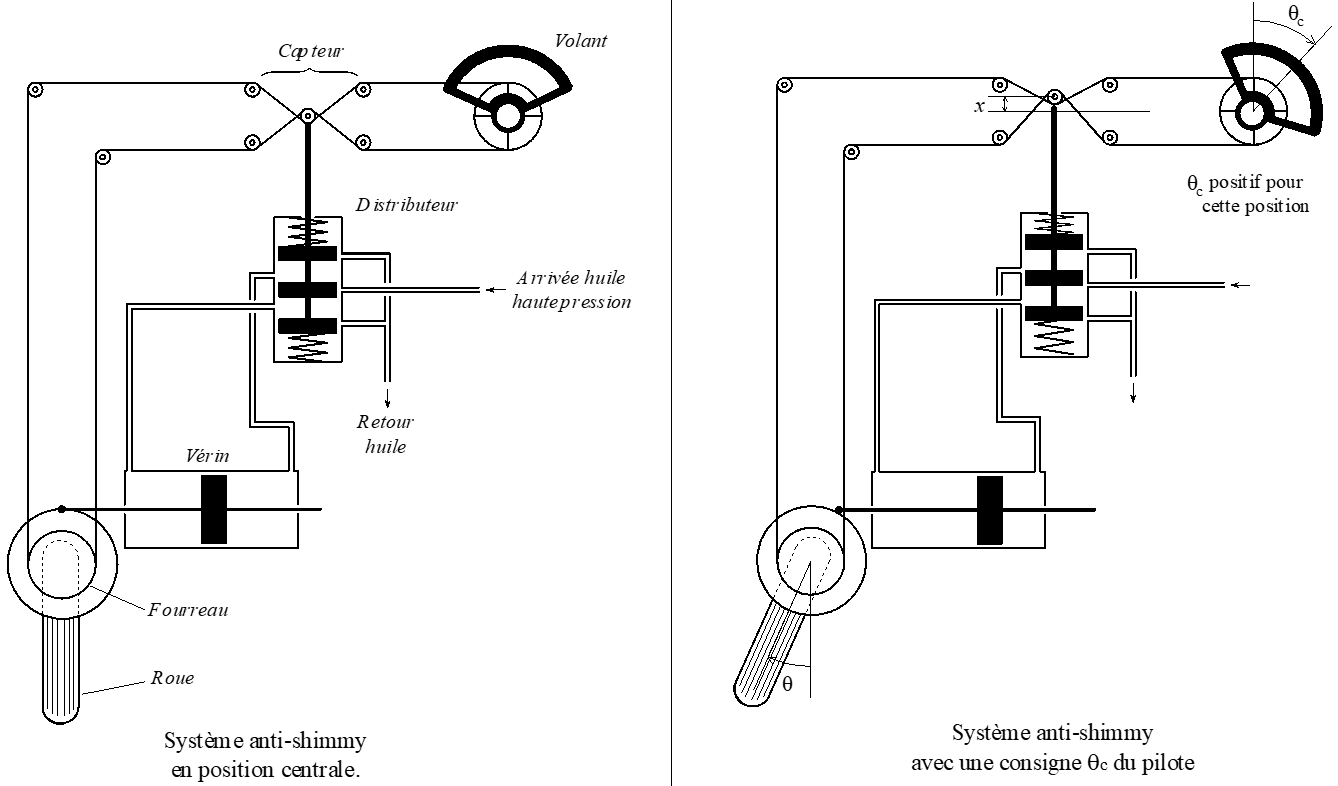
\includegraphics[width=\linewidth]{973_01}%
\end{center}


Sur le dessin siuvant, est dessiné en trait fort, la position pour $x=0$ et en trait pointillé, la position pour $x\neq0$. On note $\lambda$ la longueur $A'B$ et $\lambda_0$ la longueur $AB$. 

\begin{center}
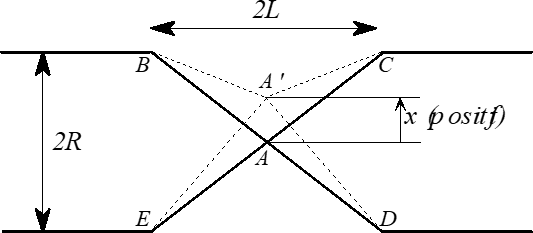
\includegraphics[width=\linewidth]{973_02}%
\end{center}


\subparagraph{}
\textit{Déterminer les valeurs de $\lambda$ et $\lambda_0$ en fonction de $R$, $L$ et $x$.}
\ifprof
\begin{corrige}
\end{corrige}
\else
\fi


\subparagraph{}
\textit{Déterminer $\lambda_0 - \lambda$ en fonction de $R$ et $\Delta \theta = \theta_c - \theta$.}
\ifprof
\begin{corrige}
\end{corrige}
\else
\fi


\subparagraph{}
\textit{En déduire une expression de $x$ en fonction de $\Delta \theta$, $R$ et $L$.}
\ifprof
\begin{corrige}
\end{corrige}
\else
\fi


\subparagraph{}
\textit{Les variations $\Delta \theta$ et $x$ sont faibles devant les autres grandeurs. Effectuer la linéarisation autour du point d’équilibre.}
\ifprof
\begin{corrige}
\end{corrige}
\else
\fi


\subparagraph{}
\textit{Déterminer la valeur de K telle que : $x=K\Delta \theta$.}
\ifprof
\begin{corrige}
\end{corrige}
\else
\fi


\begin{enumerate}
\item $\lambda_0 = \sqrt{L^2+R^2}$ et $\lambda = \sqrt{L^2 +\left(R-x^2\right)}$.
\item $2\left(\lambda_0 -\lambda\right)=R\Delta \theta$.
\item $x=R-\sqrt{R^2-R\sqrt{L^2+R^2}\Delta \theta+R^2\dfrac{\Delta \theta^2}{4}}$.
\item ...
\item $K=\dfrac{\sqrt{L^2+R^2}}{2}$.
\end{enumerate}